%\documentclass[wcp,gray]{jmlr} % test grayscale version
\documentclass[wcp]{jmlr}

% The following packages will be automatically loaded:
% amsmath, amssymb, natbib, graphicx, url, algorithm2e

%\usepackage{rotating}% for sideways figures and tables
\usepackage{longtable}% for long tables
\usepackage{array}
\usepackage{multirow}
\usepackage{color}

% The booktabs package is used by this sample document
% (it provides \toprule, \midrule and \bottomrule).
% Remove the next line if you don't require it.
\usepackage{booktabs}
% The siunitx package is used by this sample document
% to align numbers in a column by their decimal point.
% Remove the next line if you don't require it.
%\usepackage[load-configurations=version-1]{siunitx} % newer version
%\usepackage{siunitx}
%\usepackage{natbib}

% The following command is just for this sample document:
\newcommand{\cs}[1]{\texttt{\char`\\#1}}

\jmlrvolume{80}
\jmlryear{2017}
\jmlrworkshop{ACML 2017}

\title[Short Title]{IMCNN: An Identity-aware Multi-task Deep Convolutional Neural Nerwork for Face Attribute Classification}

% Use \Name{Author Name} to specify the name.
% If the surname contains spaces, enclose the surname
% in braces, e.g. \Name{John {Smith Jones}} similarly
% if the name has a "von" part, e.g \Name{Jane {de Winter}}.
% If the first letter in the forenames is a diacritic
% enclose the diacritic in braces, e.g. \Name{{\'E}louise Smith}

% Two authors with the same address
% \author{\Name{Author Name1} \Email{abc@sample.com}\and
%  \Name{Author Name2} \Email{xyz@sample.com}\\
%  \addr Address}

% Three or more authors with the same address:
% \author{\Name{Author Name1} \Email{an1@sample.com}\\
%  \Name{Author Name2} \Email{an2@sample.com}\\
%  \Name{Author Name3} \Email{an3@sample.com}\\
%  \Name{Author Name4} \Email{an4@sample.com}\\
%  \Name{Author Name5} \Email{an5@sample.com}\\
%  \Name{Author Name6} \Email{an6@sample.com}\\
%  \Name{Author Name7} \Email{an7@sample.com}\\
%  \Name{Author Name8} \Email{an8@sample.com}\\
%  \Name{Author Name9} \Email{an9@sample.com}\\
%  \Name{Author Name10} \Email{an10@sample.com}\\
%  \Name{Author Name11} \Email{an11@sample.com}\\
%  \Name{Author Name12} \Email{an12@sample.com}\\
%  \Name{Author Name13} \Email{an13@sample.com}\\
%  \Name{Author Name14} \Email{an14@sample.com}\\
%  \addr Address}


% Authors with different addresses:
\author{\Name{Author Name1} \Email{abc@sample.com}\\
	\addr Address 1
	\AND
	\Name{Author Name2} \Email{xyz@sample.com}\\
	\addr Address 2
}

\editors{Editor Name}

\begin{document}
\newcommand{\tabincell}[2]{\begin{tabular}{@{}#1@{}}#2\end{tabular}}
	
	\maketitle
	
	\begin{abstract}
		In this paper, we study the face attribute learning problem with a new perspective of considering identity information and attribute relationships simultaneously. In particular, we first introduce an Identity-aware Multi-task deep Convolutional Neural Network (IMCNN), with low-level layers shared with all attributes and high-level layers shared within attribute groups. Meanwhile, the selected feature maps are merged for an auxiliary face recognition task. IMCNN is able to learn spatial attribute relationships via grouping and inner-person attribute consistence through face recognition. Consequently, better global attribute relationships are modeled. The experimental results on CelebA and LFWA demonstrate the promise of the proposed method.
	\end{abstract}
	\begin{keywords}
		Face Attribute Learning, Multi-task Learning, Deep Learning
	\end{keywords}
	
	\section{Introduction}
	
	Face attribute learning has attracted a great attention in many real-world applications such as face identification, verification and retrieval. It aims at learning mid-level representations as the bridge between the low-level features and the high-level labels. Face attributes usually include {\em gender, race, age, hair, nose, eyes}, etc. Since such attributes provide much more informative descriptions for objects and people, they have been applied in many tasks which require detailed descriptions. For example, given low quality imagery in surveillance video, the common strategy for identity verification is to describe suspects in terms of attributes to speed up the search process. However, large-scale face attribute learning problem is still very challenging as the faces captured in the real-world are usually influenced by some factors such as illumination, pose and expression.
	
	Motivated by the success of convolutional neural network (CNN) in image classification~\cite{AlexNet,GoogleNet,fasterrcnn,fastrcnn}, the discriminative CNN representations have been widely used for face attribute learning. LNets~\cite{CelebA} are pre-trained on CelebFace~\cite{CelebFace} dataset to get a better face location for attribute prediction. In~\cite{ClassificationCNN}, a face recognition network is trained and facial features are extracted from this network to train SVMs for attribute classification. However, these identity-based methods benefit from the deep representations by CNNs, but completely ignore relationships among all the attributes and consider all the attributes independent. This is not appropriate as attribute relationships provide additional information to attribute learning and help improve the accuracy of attribute classification. For example, in gender recognition a person wearing lipstick and earrings has a high probability of being classified as a woman. Further, identity information is usually available in public dataset and real application scenarios. For the same person, some attributes are always the same such as the face shape, the mouth size and gender. An example is shown in Fig \ref{example}. We can see that the attribute Attractive is consistent for this person. 
	
	On the other hand, recent work, for example~\cite{MCNN}, considers exploiting the attribute correlations to boost the performance of attribute classification. It introduces a multi-task deep CNN (MCNN) by sharing the lower layers of the deep architectures for all the attributes and sharing the higher layers for similar attributes. MCNN assumes that many attributes are strongly related and splits all the 40 attributes into several attribute groups, where high-level layers are shared within a group and irrelevant to the rest. Although MCNN sets up the state-of-the-art in face attribute learning, it neglects attribute relationships related to the identity information, since attributes are highly correlated within the same person but less correlated among different identities.
	
	In this paper we investigate the face attribute learning problem with a new perspective of considering identity information and attribute relationships simultaneously. We hypothesize that combining identity information and attribute relationship modeling together enables us to develop more accurate attribute learning algorithms. Our hypothesis is based on the following insights: (1) most attributes show consistency for the same identity while attributes from different persons are independent; (2) by performing face recognition on attribute features, these inner-person attribute relationships can be modeled, since identity information forces attribute features to be similar for the same person.
	
	We present an Identity-aware Multi-task deep Convolutional Neural network (IMCNN), a novel deep learning framework, which performs identity recognition and attribute classification in a single framework. IMCNN exploits all the attributes and identity information by sharing lower layers of IMCNN for all attributes, sharing higher layers of IMCNN for strongly correlated attributes, and performing identity recognition in the merged higher layer.
	
	In particular, all the attributes are split into several attribute groups according to spatial information and the selected feature maps of the attribute groups are merged to perform face recognition. The grouping scheme encourages IMCNN modeling the spatial attribute relationships, while the loss function of face recognition can be considered as a regularization term to model inner-person attribute consistency, since the merged features of the same person are forced to be close in the feature space, which leads to similar attribute predictions for the same person. Consequently, combining spatial attribute relationships and inner-person attribute consistency, IMCNN is capable of modeling better global attribute relationships. Extensive evaluations are conducted to investigate the performances of IMCNN. The experimental results on CelebA~\cite{CelebA} as well as LFWA~\cite{LFW} validate the superior performance of it.
	
	\section{Related Work}
	Attribute classification often extracts features from landmarks or facial parts~\cite{POOF,poselet,2009attribute,panda}. Hand-picked facial regions are used for learning AdaBoost-based features for each attribute in~\cite{2009attribute}, which are fed into independent SVMs for a final prediction. In~\cite{POOF}, HOG features are extracted from facial parts located by landmarks, where a single SVM is trained for each attribute to perform attribute classification. ~\cite{poselet} collects body parts with different poses and HOG-like features are learned from these poselets; then, SVMs are trained as classifiers.
	
	Thanks to the great breakthrough of deep learning~\cite{AlexNet,GoogleNet,VGGNet,fastrcnn,fasterrcnn,CelebA,ClassificationCNN,AFFACT}, high-level features can be extracted from the whole image without landmarks or parts information. ~\cite{ClassificationCNN} extracts features at different layers of a face recognition CNN. These features are used as training data for linear SVM to generate attribute scores. ~\cite{CelebA} localizes face by training two cascade LNets and then extracting the 40 features for the 40 attributes via an ANet. Finally, 40 SVMs are trained for the 40 attributes.
	
	Though most deep-learning methods do not rely on landmarks or parts, they consider attributes to be independent. Using independent SVMs as classifiers, they are not able to model attribute relationships, which are crucial for attribute prediction. In addition, all the previous methods do not make full use of the available identity information, which has been proven closely related with attribute learning.
	
	\section{Method}
	\subsection{IMCNN Architecture}
	Multi-task learning~\cite{multi1,multi2,multi3,multi4,multi5} aims at learning multiple tasks simultaneously. It assumes that related tasks should be correlated via a certain structure. This is especially true for face attribute learning with deep architectures as there is a hierarchy of attributes, which should be related through shared low-level features. Meanwhile, the high-level features are still task-specific to retain the differently discriminative information for different attribute tasks.
	
	\begin{figure}[htb]
		\begin{center}
			\centering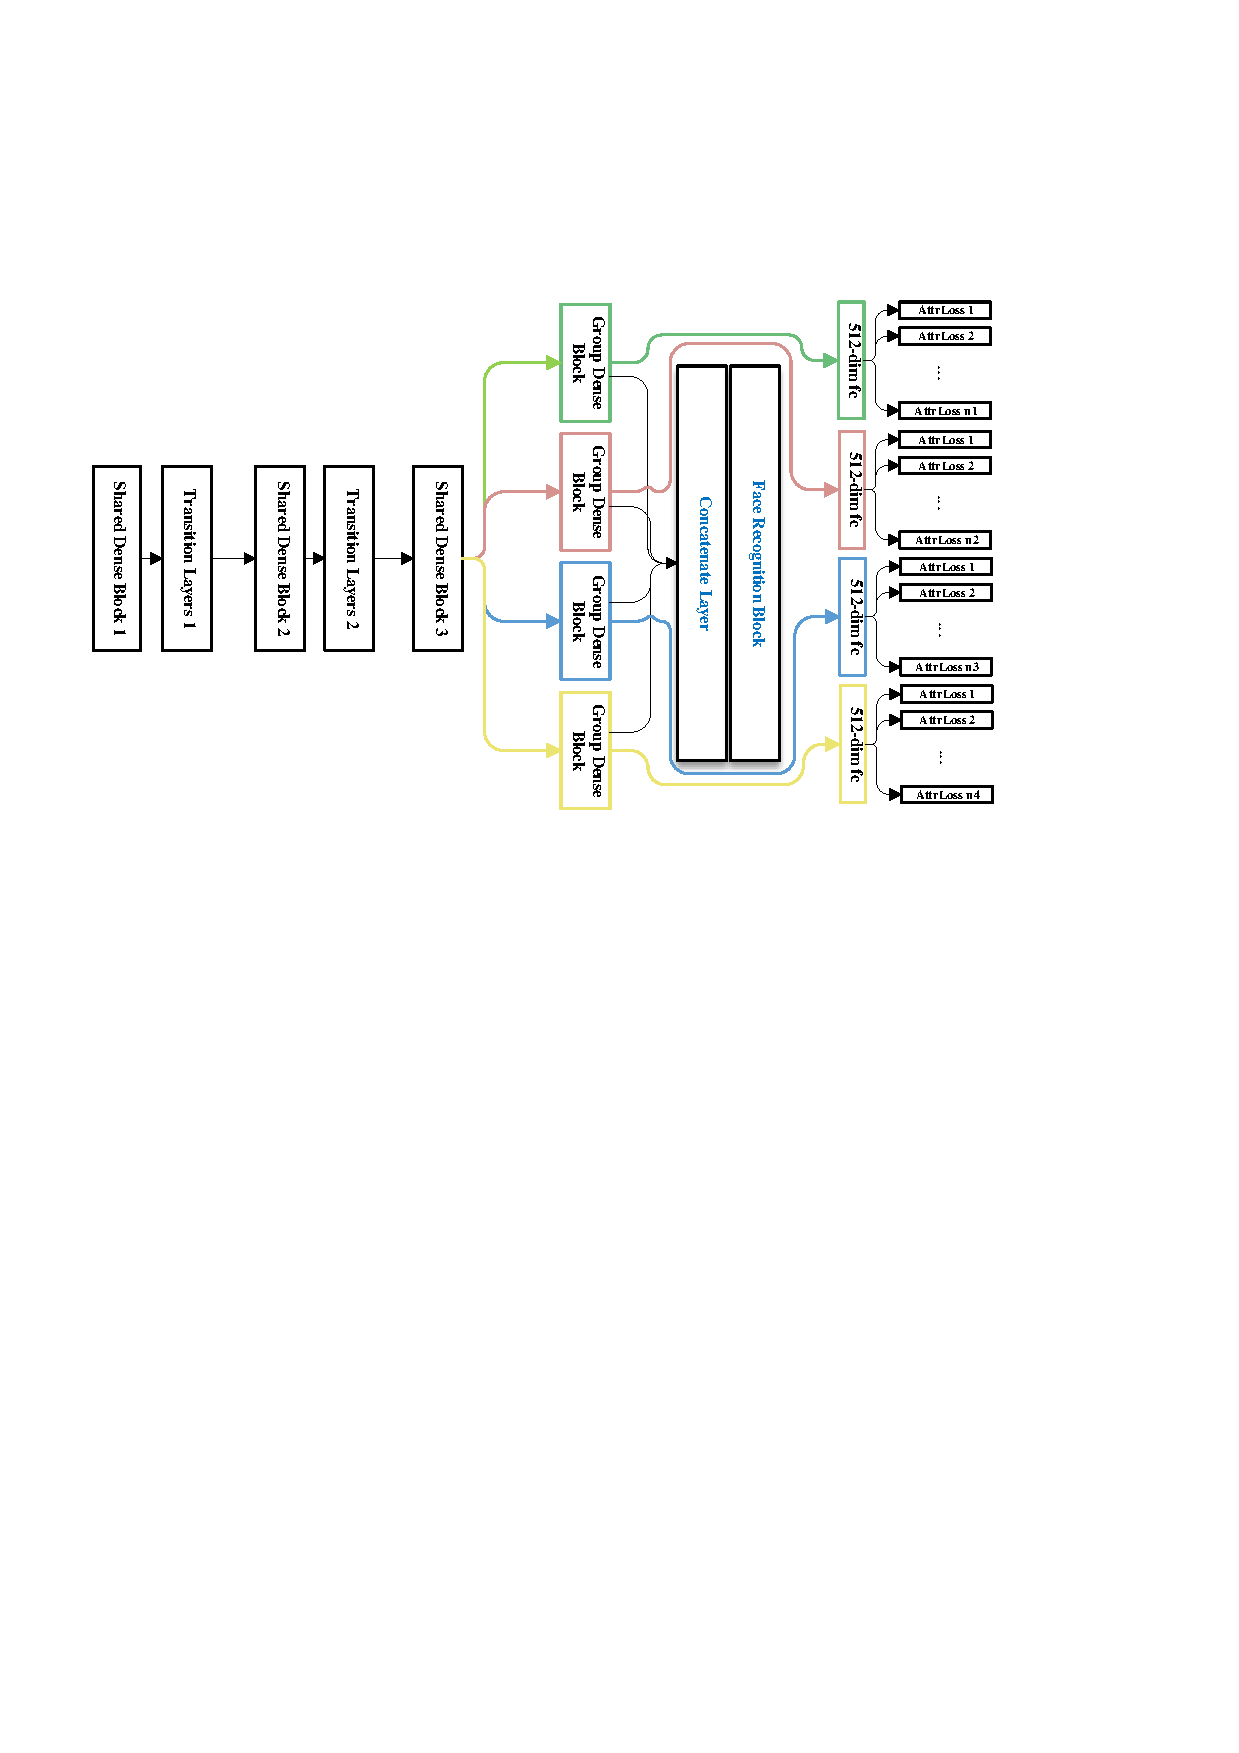
\includegraphics[width=16cm]{new_imgs/DenseNet.pdf}
			\label{fig:long}
		\end{center}
		\caption{Architecture of IMCNN.}
		\label{IMCNN_Arch}
	\end{figure}
	
	In this section, we investigate the attribute learning problem with the multi-task learning scenario. In particular, we propose to share low-level features for all tasks and to share high-level features for similar tasks. For CNNa, it is natural to bifurcate them so that all the layers before the bifurcation are shared by all the attributes and the layers after the bifurcation are shared within strongly related attributes. Besides, since the identity information of samples usually exists in the training data, we develop face recognition tasks from the same data as an auxiliary task, forcing the attribute learning and identity recognition to benefit from each other. Consequently, we propose IMCNN to improve the generalization performance of multi-task attribute learning.
	
	Fig.\ref{IMCNN_Arch} illustrates the architecture of IMCNN. Low-level layers from Conv1 to Pool3 are shared by all the 40 attributes. After that, group strategy is used to separate layers. There are 6 groups according to locations after the first split: Nose, Mouth, Eyes, Face, Gender and Rest; then, the Rest group is further separated into 4 smaller groups in the second split: AroundHead, FacialHair, Cheeks and Fat. Further, we merge the 6 attribute groups by concatenating the feature maps, which are the inputs of our face recognition task. This split-and-merge structure efficiently combines the two tasks by using rich spatial information from attribute classification for face recognition. In addition, attribute relationships are explicitly learned by separating attributes based on their similarities into groups. Grouping configuration follows~\cite{MCNN}, as shown bellow and we list hyper-parameters of IMCNN in Table \ref{IMCNN net}.
	
	\textbf{Upper Group:} \emph{Arched Eyebrows, Bags Under Eyes, Bushy Eyebrows, Narrow Eyes, Eyeglasses, Black Hair, Blond Hair, Brown Hair, Gray Hair, Balding, Receding Hairline, Bangs,  Wearing Hat}.
	
	\textbf{Middle Group:} \emph{Big Nose, Pointy Nose, Wearing Earrings, Sideburns, High Cheekbones, Rosy Cheeks}.
	
	\textbf{Lower Group:} \emph{Big Lips, Lipsticks, Mouth Slightly Open, Wearing Necklace, Wearing Necktie, Mustache, No Beard, Goatee, Double Chin}.
	
	\textbf{Whole Image Group:} \emph{Male, Smiling, Attractive, Blurry, Oval Face, Pale Skin, Young, Heavy Makeup, Straight Hair, Wavy Hair, 5 o'Clock Shadow, Chubby}.
	
	\begin{table}[htb]
		\begin{center}
			\begin{tabular}{|c|c|c}
				\hline
				Layers & Output Size & IMCNN \\
				\hline
				\multirow{2}{*}{Stem}
				& $112\times112$ &  $7\times7$ conv, s=2 \\
				\cline{2-3}
				 & $56\times56$ &  $3\times3$ max pool, s=2 \\
				\hline
				\multirow{2}{*}{Shared Dense Block(1)}
				& \multirow{2}{*}{$56\times56$} & \multirow{2}{*}{\tabincell{c}{$1\times1$ conv \\ $3\times3$ conv} $\times4$} \\
				 & & \\
				 \hline
				 \multirow{2}{*}{Transition Layers(1)}
				 & $56\times56$ &  $1\times1$ conv \\
				 \cline{2-3}
				 & $28\times28$ &  $2\times2$ ave pool, s=2 \\
				 \hline
				 \multirow{2}{*}{Shared Dense Block(2)}
				 & \multirow{2}{*}{$28\times28$} & \multirow{2}{*}{\tabincell{c}{$1\times1$ conv \\ $3\times3$ conv} $\times8$} \\
				 & & \\
				 \hline
				 \multirow{2}{*}{Transition Layers(2)}
				 & $28\times28$ &  $1\times1$ conv \\
				 \cline{2-3}
				 & $14\times14$ &  $2\times2$ ave pool, s=2 \\
				 \hline
				 \multirow{2}{*}{Shared Dense Block(3)}
				 & \multirow{2}{*}{$14\times14$} & \multirow{2}{*}{\tabincell{c}{$1\times1$ conv \\ $3\times3$ conv} $\times16$} \\
				 & & \\
				 \hline
				 \multirow{2}{*}{Group Dense Block}
				 & \multirow{2}{*}{$14\times14$} & \multirow{2}{*}{\tabincell{c}{$1\times1$ conv \\ $3\times3$ conv} $\times4$} \\
				 & & \\
				 \hline
				 \multirow{5}{*}{Face Recognition Block}
				 & $14\times14$ & maxout \\
				 \cline{2-3}
				 & \multirow{2}{*}{$14\times14$} & \multirow{2}{*}{\tabincell{c}{$1\times1$ conv \\ $3\times3$ conv} $\times4$} \\
				 & & \\
				 \cline{2-3}
				 & $512$-dim & fc \\
				 \cline{2-3}
				 & $1$-dim & softmax loss \\
				 \hline
			\end{tabular}
		\end{center}
		\caption[short]{Aechitecture of IMCNN. Batch normalization~\cite{BatchNorm} and ReLU~\cite{ReLU} are adopted after each convolutional layer.}
		\label{IMCNN net}
	\end{table}
	
	\begin{table}[htb]
		\begin{center}
			\begin{tabular}{|c|c|c|c}
				\hline
				Layer & Kernel Size & Output Size \\
				\hline
				Conv1 & $\tiny{3\times3\times64}$ & $\tiny{112\times112\times64}$ \\
				\hline
				Pool1 & $\tiny{2\times2}$ & $\tiny{56\times56\times64}$ \\
				\hline
				Conv2a & $\tiny{3\times3\times64}$ & $\tiny{56\times56\times64}$ \\
				\hline
				Conv2 & $\tiny{3\times3\times192}$ & $\tiny{56\times56\times192}$ \\
				\hline
				Pool2 & $\tiny{2\times2}$ & $\tiny{28\times28\times192}$ \\
				\hline
				Conv3a & $\tiny{3\times3\times192}$ & $\tiny{28\times28\times192}$ \\
				\hline
				Conv3 & $\tiny{3\times3\times384}$ & $\tiny{28\times28\times384}$ \\
				\hline
				Pool3 & $\tiny{2\times2}$ & $\tiny{14\times14\times384}$ \\
				\hline
				ConvAttr & $\tiny{3\times3\times512}$ & $\tiny{7\times7\times512}$ \\
				\hline
				FC1Attr & $\tiny{1024}$ & $\tiny{1\times1\times1024}$ \\
				\hline
				FC2Attr & $\tiny{1024}$ & $\tiny{1\times1\times1024}$ \\
				\hline
			\end{tabular}
		\end{center}
		\caption[short]{Aechitecture of IMCNN. Batch normalization~\cite{BatchNorm} and ReLU~\cite{ReLU} are adopted after each convolutional layer.}
		\label{IMCNN net}
	\end{table}
	
	\subsection{Joint Optimization of Attributes and Identities}
	Multiple loss functions are employed when there are multiple tasks to be learned in a neutal network~\cite{yolo9000,liu2016ssd,long2015fully}. Therefore, we jointly optimize attribute classification and face recognition via combining two loss functions, namely, $Loss_{ID}$ and $Loss_{ATTR}$. $Loss_{ATTR}$ is the sum of the losses of all the attributes. For the $i$-th attribute, we formulate its loss as follows:
	
	\begin{equation*}
	loss_{i} = \frac{1}{N}\sum_{n=1}^N\{[p_{n}log[\sigma(f_{g(i)})] + (1-p_{n})log[1-\sigma(f_{g(i)})] ]\},
	\end{equation*}
	where N indicates batch size, $p_{n}$ is a binary label, which is assigned as 1 when a face has the corresponding attribute or 0 otherwise, $\sigma$ is sigmoid function $\sigma(x) = \frac{1}{1+e^{-x}}$, and $f(j)$ represents the output of the FC2Attr layer of the $j$-th group. The $g(i)$ function returns the group index for each attribute index. For example, since the attribute Male belongs to the group Gender, we have $g(1)=2$ when the attribute index of Male is 1 and the group index of Gender is 2. Note that the value range of $g(i)$ varies from 1 to 9, since we have 9 different FC2Attr layers, which significantly reduces the model complexity while learning the task-specific parameters for all the attributes. Then, we compute \emph{Loss$_{ATTR}$} by summing over $loss_{i}$ as follows:
	
	\begin{equation*}
	Loss_{ATTR} = \sum_{i=1}^{T}{loss_i},
	\end{equation*}
	where $T$ is the number of the attributes.
	
	By merging features from different attribute groups, we can compute \emph{Loss$_{ID}$} on the merged features:
	
	\begin{equation*}
	\begin{split}
	Loss_{ID} = -log(\hat{p}_{k}), \hat{p}_{k} = \frac{h(F)_k}{\sum_{n=1}^{N}{h(F)_n}}, k \in{[1, N]},
	\end{split}
	\end{equation*}
	where $F$ is the merged features. In IMCNN, 6 ConvAttr output feature maps are concatenated to get $F$; $h(\cdot)$ represents a fully connected mapping between $F$ and an N-dimensional vector. $\hat{p_k}$ is the predicted probability of the $k$-th identity and is computed from $h(F)$ in a softmax function. Finally, $LOSS$ of our IMCNN network is the weighted sum of $Loss_{ID}$ and $Loss_{ATTR}$ as follows:
	
	\begin{equation}
	LOSS = Loss_{ATTR} + \lambda\times Loss_{ID},
	\label{LOSS}
	\end{equation}
	where $Loss_{ID}$ acts like a regularization term, which improves the generalization power of IMCNN and makes it more robust. As shown in Sec. 3, the choice of $\lambda$ is essential for the performance of IMCNN.
	
	Under the regularization of $Loss_{ID}$, the strength of the joint optimization in Eq.(\ref{LOSS}) lies on two aspects. First, the identity information and attributes are complementary in the process of learning face representations. Attributes usually respond to local facial parts, while the identity information provides a global constraint via $Loss_{ID}$. Therefore, as shown in Fig 2 IMCNN is able to learn fine-grained feature maps. Second, regularized by $Loss_{ID}$, IMCNN can model better attribute relationships by exploiting inner-person attribute correlations. In particular, attributes are consistent for the same person. For example, as illustrated in Fig. \ref{attr_corr}, we make attribute correlation analysis on a collection of 35 images within a person and among different identities respectively. It indicates that most images of the same person have similar attribute labels, while attributes for different identities are relatively independent. $Loss_{ATTR}$ fails to model this inner-person attribute correlations as it treats every image independently, while $Loss_{ID}$ forces the merged feature maps $F$ to be as similar as possible for the same person via performing face recognition on $F$. Since $F$ consists of feature maps from all the attribute groups, predictions for all the attributes are likely to be similar for the same person.
	\begin{figure}[htb]
		\begin{center}
			\centering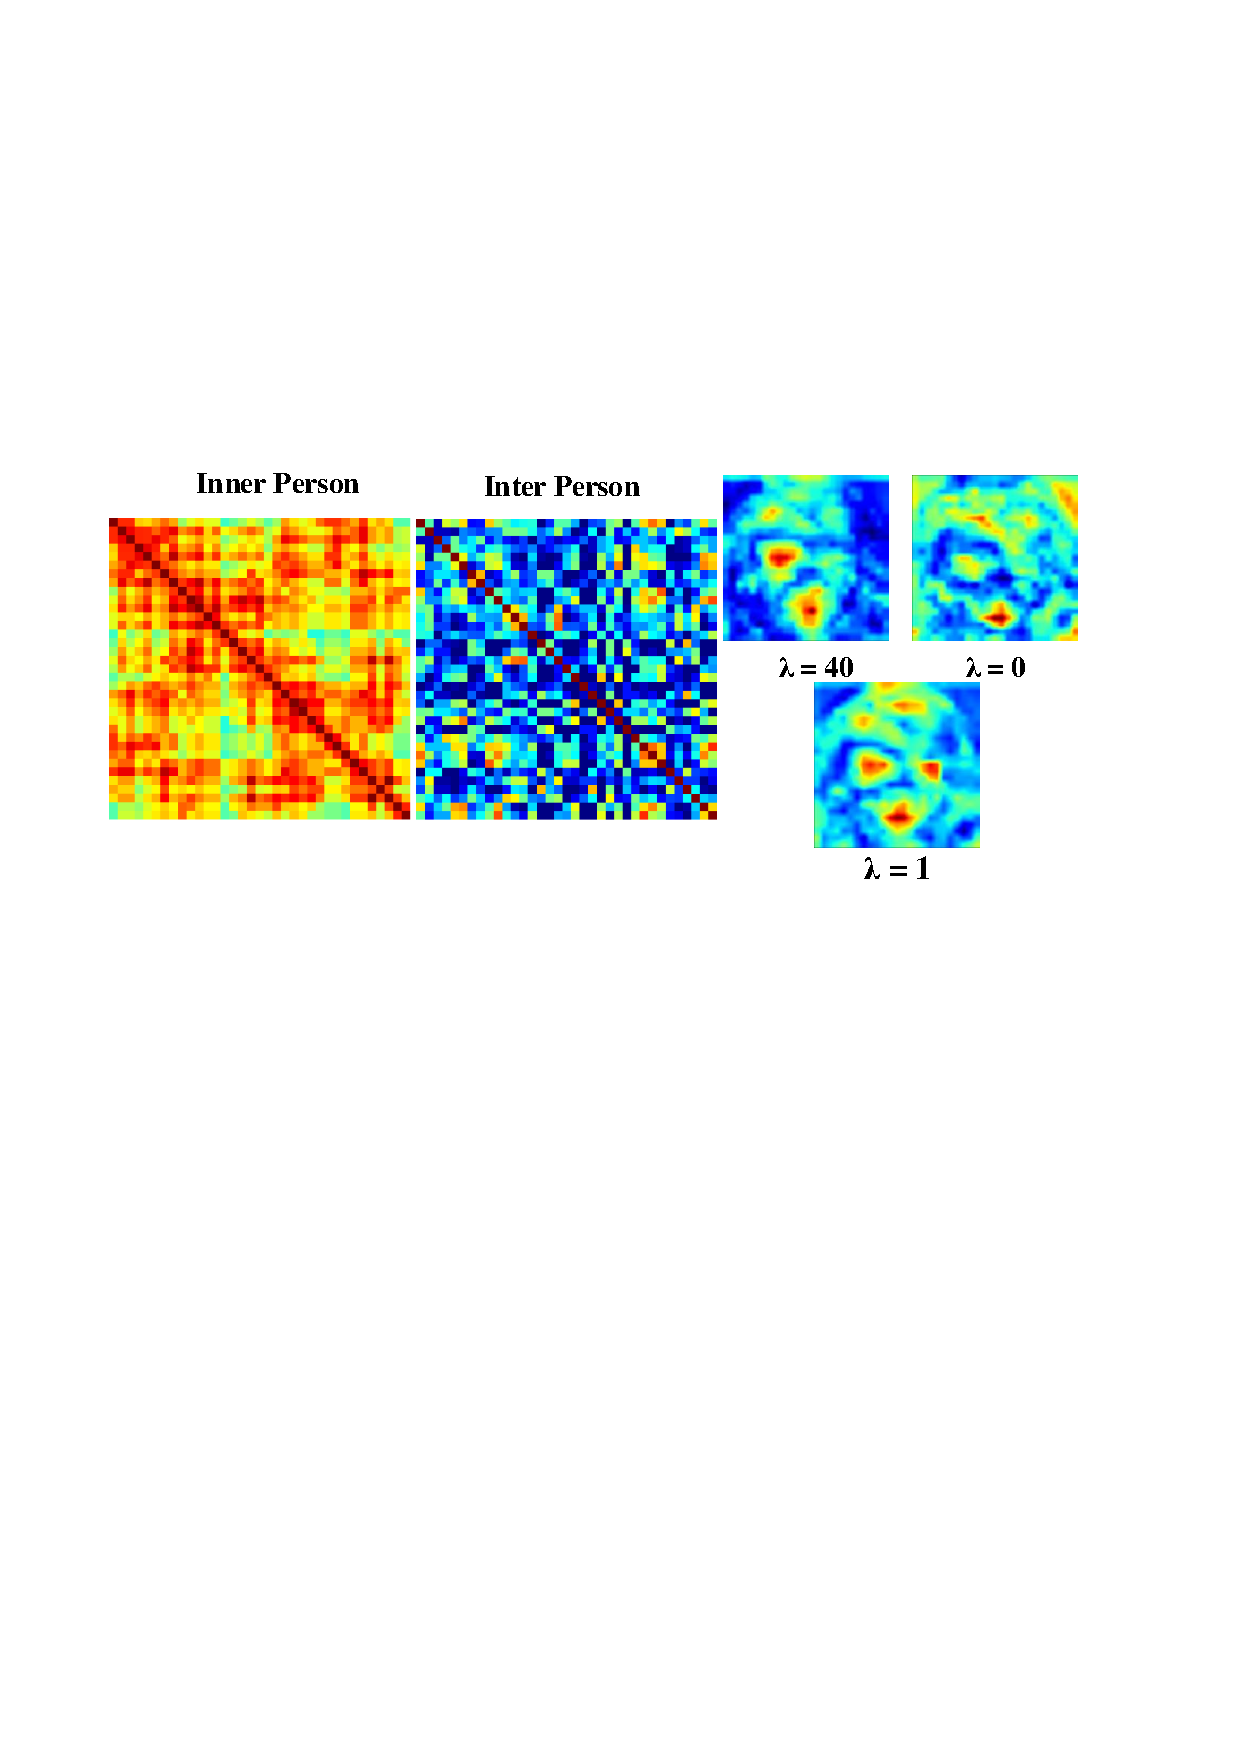
\includegraphics[width=16cm]{./new_imgs/CorrelationAndFeature.pdf}
		\end{center}
		\caption[short]{Correlation Analysis and feature maps of IMCNN with different $\lambda$ values.}
		\label{attr_corr}
	\end{figure}
	
	%------------------------------------------------------------------------
	\section{Experiment}
	
	\subsection{Experimental Configurations}
	
	A large face dataset with identity and attribute labels is needed for training IMCNN. One option is LFW, consisting of 13,323 images from 5,749 identities. However, since many identities only have 1 image in LFW, it is not suitable for jointly training with attribute classification and face recognition tasks. While CelebA~\cite{CelebA} has 202,599 images of 10,000 persons, each person has 20 images on average. Consequently, we consider CelebA as our training set for IMCNN and its identity information is public available.
	
	We split the CelebA into two parts, one for training and another for test. The training set contains ~180,000 images of ~8,000 identities while the test set contains ~20,000 images from the rest identities. Note that the training set doesn't share identities with the test set. Therefore, IMCNN needs to model a general relationship between identity information and attributes, so that it can perform well on new identities.
	
	We train all the models in the Caffe~\cite{Caffe} framework on single GTX1080ti graphic card. For our IMCNN, we use a batch size of 64 and a initial learning rate of 0.001 with the SGD strategy. We further decrease the learning rate two times after every 10 epoches. All the filters of convolutional layers and fully connected layers are initialized with the xavier method. During the test process, we resize the images to $112 \times 112$ and feed them into the models. Different from the training process, which requires identity information, the test process only requires a face image. We report accuracies on both the test set of CelebA and the whole LFWA dataset.
	
	\subsection{Baselines}
	
	To verify the effectiveness of IMCNN, we compare them with the state-of-the-art methods: LNets+ANet~\cite{CelebA}, face attribute prediction with classification CNN (referred as ID Net)~\cite{ClassificationCNN} and multi-task convolutional neural network (referred as MCNN)~\cite{MCNN}. Further, we also study different configurations of IMCNN. Specifically, we train an ATTR Net, which is optimized with $Loss_{ATTR}$ only. IMCNNs with different $\lambda$ values are also trained to explore the influence of the identity information. For methods with public available results including LNets+ANet, ID Net and MCNN, we report the public results. For ATTR Net, we train it with the same configurations as the IMCNN for fair comparisons.
	
	\begin{table*}
		\tiny
		\begin{center}
			\renewcommand\arraystretch{1.8}
			\begin{tabular}{c|c|c|c|c|c||c|c|c|c|c|}
				\hline
				& LNets+ANet & ID Net & MCNN & ATTR Net & IMCNN & LNets+ANet & ID Net & MCNN & ATTR Net & IMCNN \\
				\hline
				5 Shadow & 91 & 92.64 & 94.41 & 94.87 & \textbf{95.43} & 84 & 85.32 & 77.70 & 77.89 & \textbf{85.11} \\
				\hline
				Arch. Eyebrows & 79 & 82.03 & 83.55 & 83.33 & \textbf{84.99} & 82 & 84.58 & 82.36 & 82.11 & \textbf{83.19} \\
				\hline
				Attractive & 81 & 79.99 & 82.94 & 82.74 & \textbf{83.71} & 83 & 82.16 & 80.42 & 80.26 & \textbf{84.52} \\
				\hline
				Bags Un. Eyes & 79 & 81.43 & 84.98 & 85.63 & \textbf{86.21} & 83 & 87.31 & 83.51 & 84.00 & \textbf{86.37} \\
				\hline
				Bald & 98 & 97.16 & 98.87 & 98.82 & \textbf{99.19} & 88 & 86.99 & 91.99 & 91.85 & \textbf{92.17} \\
				\hline
				Bangs & 95 & 94.64 & 96.04 & 96.02 & \textbf{96.71} & 88 & 88.13 & 89.99 & 89.99 & \textbf{91.03} \\
				\hline
				Big Lips & 68 & 68.87 & 71.20 & 70.98 & \textbf{72.77} & 75 & 75.68 & 79.21 & 78.33 & \textbf{82.37} \\
				\hline
				Big Nose & 78 & 82.39 & 84.50 & 84.63 & \textbf{85.66} & 81 & 83.67 & 84.67 & 84.99 & \textbf{86.11} \\
				\hline
				Black Hair & 88 & 84.14 & 89.87 & 89.73 & \textbf{90.81} & 90 & 88.56 & 92.35 & 92.16 & \textbf{92.52} \\
				\hline
				Blond Hair & 95 & 94.22 & 95.97 & 95.76 & \textbf{96.55} & 97 & 95.89 & 97.45 & 97.10 & \textbf{98.02} \\
				\hline
				Blurry & 84 & 95.75 & 96.08 & 96.12 & \textbf{96.86} & 74 & 83.67 & 85.30 & 85.38 & \textbf{86.83} \\
				\hline
				Brown Hair & 80 & 83.54 & 88.99 & 88.85 & \textbf{90.07} & 77 & 79.47 & 80.94 & 80.99 & \textbf{81.55} \\
				\hline
				Bushy Eyebrows & 90 & 92.20 & 92.80 & 92.63 & \textbf{93.50} & 82 & 83.68 & 85.11 & 85.13 & \textbf{85.32} \\
				\hline
				Chubby & 91 & 92.89 & 95.66 & 95.68 & \textbf{96.47} & 73 & 75.84 & 76.90 & 76.96 & \textbf{77.83} \\
				\hline
				Double Chin & 92 & 94.36 & 96.41 & 96.42 & \textbf{97.22} & 78 & 80.09 & 81.17 & 81.17 & \textbf{96.33} \\
				\hline
				Eyeglasses & 99 & 99.25 & 99.63 & 99.64 & \textbf{99.80} & 95 & 94.87 & 91.22 & 91.20 & \textbf{96.33} \\
				\hline
				Goatee & 95 & 95.77 & 97.30 & 97.29 & \textbf{97.74} & 78 & 79.36 & 82.52 & 82.54 & \textbf{83.77} \\
				\hline
				Gray Hair & 97 & 97.28 & 98.20 & 98.16 & \textbf{98.47} & 84 & 83.69 & 89.04 & 89.00 & \textbf{90.63} \\
				\hline
				Heavy Makeup & 90 & 88.58 & 91.34 & 91.41 & \textbf{92.47} & 95 & 93.11 & 95.84 & 96.00 & \textbf{96.13} \\
				\hline
				H. Cheekbones & 87 & 84.21 & 87.55 & 87.49 & \textbf{88.43} & 87 & 84.52 & 88.25 & 88.15 & \textbf{88.38} \\
				\hline
				Male & 98 & 97.32 & 98.16 & 98.18 & \textbf{98.69} & 94 & 93.66 & 93.66 & 93.74 & \textbf{94.73} \\
				\hline
				Mouth S. O. & 92 & 92.03 & 93.74 & 93.70 & \textbf{94.79} & 82 & 81.87 & 83.47 & 83.44 & \textbf{84.25} \\
				\hline
				Mustache & 95 & 95.11 & 96.93 & 96.84 & \textbf{97.45} & 92 & 92.36 & 93.53 & 93.48 & \textbf{94.02} \\
				\hline
				Narrow Eyes & 81 & 86.04 & 87.16 & 87.24 & \textbf{88.25} & 81 & 81.59 & 82.37 & 82.49 & \textbf{83.17} \\
				\hline
				No Beard & 95 & 95.69 & 96.11 & 96.25 & \textbf{97.70} & 79 & 80.21 & 82.13 & 82.25 & \textbf{82.68} \\
				\hline
				Oval Face & 66 & 70.15 & 75.81 & 75.12 & \textbf{76.90} & 74 & 75.39 & 77.38 & 76.98 & \textbf{77.62} \\
				\hline
				Pale Skin & 91 & 94.91 & 97.01 & 96.90 & \textbf{97.76} & 84 & 87.22 & 93.41 & 93.35 & \textbf{94.52} \\
				\hline
				Receed. Hairline & 89 & 92.37 & 93.81 & 93.76 & \textbf{94.74} & 85 & 85.39 & 86.26 & 86.24 & \textbf{87.12} \\
				\hline
				Rosy Cheeks & 90 & 93.28 & 95.13 & 95.11 & \textbf{95.87} & 85 & 85.39 & 86.26 & 86.24 & \textbf{87.12} \\
				\hline
				Pointy Nose & 72 & 74.62 & 77.47 & 77.32 & \textbf{78.67} & 78 & 83.52 & 87.52 & 87.46 & \textbf{87.15} \\
				\hline
				Sideburns & 96 & 95.58 & 97.82 & 97.84 & \textbf{97.14} & 77 & 76.33 & 82.73 & 82.79 & \textbf{84.07} \\
				\hline
				Smiling & 92 & 91.57 & 92.66 & 92.92 & \textbf{93.73} & 91 & 90.17 & 91.75 & 91.99 & \textbf{92.07} \\
				\hline
				Straight Hair & 73 & 78.38 & 83.39 & 83.24 & \textbf{85.09} & 76 & 77.32 & 78.72 & 78.64 & \textbf{79.35} \\
				\hline
				Wavy Hair & 80 & 75.88 & 83.92 & 83.49 & \textbf{85.38} & 76 & 75.39 & 81.96 & 81.48 & \textbf{83.01} \\
				\hline
				Wear. Earings & 82 & 85.73 & 90.32 & 90.70 & \textbf{91.76} & 94 & 93.02 & 94.71 & 95.00 & \textbf{95.08} \\
				\hline
				Wear. Hat & 99 & 98.87 & 99.04 & 99.01 & \textbf{99.33} & 88 & 89.64 & 90.20 & 90.11 & \textbf{90.80} \\
				\hline
				Wear. Lipstick & 93 & 90.45 & 93.95 & 94.21 & \textbf{94.76} & 95 & 92.07 & 94.89 & 95.12 & \textbf{95.24} \\
				\hline
				Wear. Necklace & 71 & 85.01 & 86.82 & 87.03 & \textbf{87.91} & 88 & 88.59 & 89.66 & 90.01 & \textbf{90.11} \\
				\hline
				Wear. Necktie & 93 & 91.13 & 96.53 & 96.55 & \textbf{97.33} & 79 & 78.82 & 80.50 & 80.56 & \textbf{81.36} \\
				\hline
				Young & 87 & 84.56 & 88.48 & 88.70 & \textbf{89.65} & 86 & 84.26 & 85.37 & 85.67 & \textbf{86.11} \\
				\hline
				Average& 87 & 88.75 & 91.25 & 91.26 & \textbf{92.16} & 84 & 84.64 & 86.27 & 86.25 & \textbf{87.38} \\
				\hline
			\end{tabular}
		\end{center}
		\caption{Performance comparison. Left columns show the performance on CelebA. Right ones give that of LFWA.}
		\label{results}
	\end{table*}
	
	\textbf{Sensitivity of $\lambda$:} To verify the effectiveness of the auxiliary face recognition task, we train IMCNN with different $\lambda$ values. Note that we refer IMCNN with a zero $\lambda$ to ATTR Net. As illustrated in Fig \ref{Loss}, accuracy under different $\lambda$ values varies and achieves the best when $\lambda$ equals 1. Interestingly, accuracy drops dramatically when $\lambda$ increases or decreases. Further, a properly chosen $\lambda$ value encourages IMCNN to reach significantly lower training and validation losses. As we can see in Fig \ref{Loss}, the validation loss drops from $15$ to $14$ when $\lambda$ increases from 0 to 1. And it drops from $16$ to $14$ when $\lambda$ decreases from 40 to 1. The change of accuracy and loss can be explained when $Loss_{ID}$ is interpreted as a regularization term to the attribute classification task. Since $Loss_{ID}$ forces feature maps of the same person to be as close as possible, a proper $\lambda$ helps IMCNN to force features of the same person to be close. As a result, a higher performance is obtained as the inner-person consistency is modeled. However, when $\lambda$ is too large, IMCNN is not able to model attribute diversity for the same person, so that the performance is harmed. On the other hand, when $\lambda$ is too small, the regularization influence of the identity information is limited.
	
	\begin{figure}[htb]
		\begin{center}
			\centering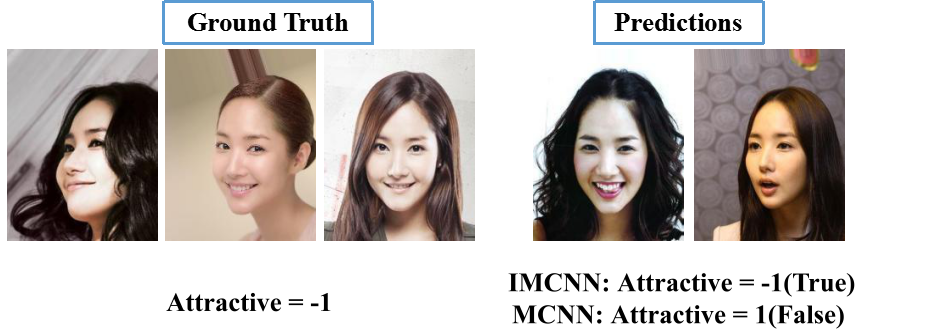
\includegraphics[width=16cm]{./new_imgs/attractive_8.png}
		\end{center}
		\caption{An example illustrates the inner-person attribute consistency. IMCNN takes advantage of the identity information while MCNN fails to make the right predictions.}
		\label{example}
	\end{figure}
	
	\textbf{Comparison with other methods:} According to our experimental results in Table \ref{results}, IMCNN achieves an average accuracy of 92.16\%, surpassing all the other methods by a large margin. On the one hand, IMCNN outperforms identity-based methods including LNets+ANet and ID Net, especially on FacialHair and AroundHead groups. We attribute this to their pre-training on face recognition, which forces them putting more weights to identity-related facial parts while decreasing its attention on facial hair as well as around head areas. On the contrary, face recognition is an auxiliary task in IMCNN. By choosing proper $\lambda$, $Loss_{ID}$ does not harm identity-free attributes but helps model inner-person attribute consistency. On the other hand, IMCNN beats MCNN and ATTR Net on every single attribute, which implies that identity is informative for all the 40 attributes. We attribute this to the supervision of the identity information. In Fig \ref{example}, IMCNN takes advantage of the identity information while MCNN fails to make the right predictions. To better understand this phenomenon, we compare feature maps from Conv3 of IMCNN with ATTR Net in Fig \ref{attr_corr}. We find that ATTR Net puts more weights on facial hair and around head areas, since nearly half of the 40 attributes lie in these areas. But these areas are large and easily polluted by noise and occlusion. Nevertheless, IMCNN learns more fine-grained feature maps putting more weights on facial parts while leaving small regions of responses on identity-free areas such as hair and forehead. As a result, IMCNN directly enhances the performance on identity-related groups including Nose Group and Eyes Group. In the meantime, it indirectly boosts the performance of identity-free groups by decreasing the possibility of being influenced by noise, illumination and other factors. Therefore, the accuracies on both identity-related attributes and identity-free attributes are improved significantly.
	\begin{figure}[htb]
		\begin{center}
			\centering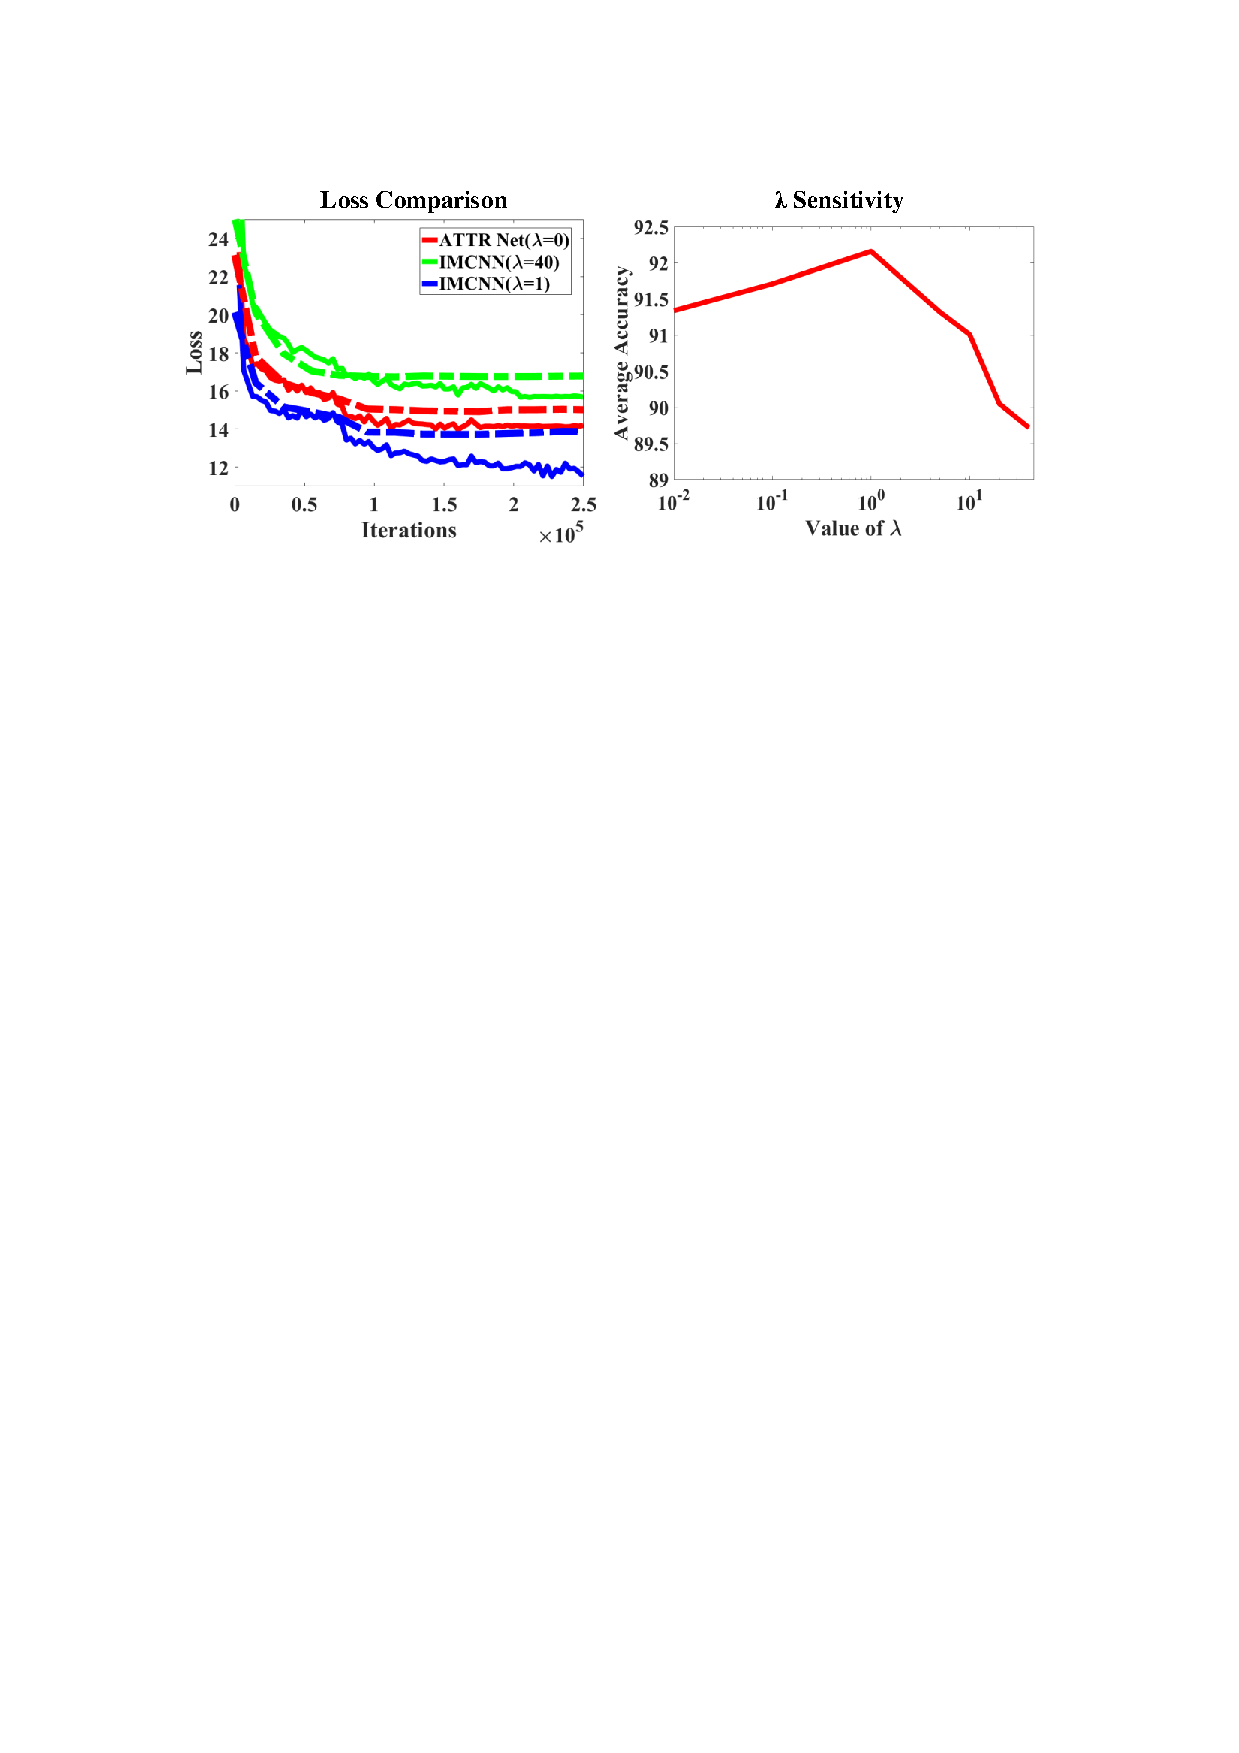
\includegraphics[width=16cm]{./new_imgs/LossAndSensitivity_crop.pdf}
		\end{center}
		\caption{Loss comparison and accuracy under different $\lambda$ values. The dotted lines represent the validation loss.}
		\label{Loss}
	\end{figure}
	
	\section{Conclusion}
	In this paper, we investigate the face attribute learning problem from a new perspective of considering the identity information and attribute relationships simultaneously. In particular, we introduce an Identity-aware Multi-task deep Convolutional Neural Network (IMCNN), with low-level layers shared by all attributes and high-level layers shared within attribute groups. Meanwhile, the selected feature maps are merged for an auxiliary face recognition task, to model the inner-person consistency. The experimental results on CelebA and LFWA demonstrate the promise of the proposed methods.
	
	%\bibliographystyle{plain}
	\bibliography{acml17}
	
\end{document}
